% \usepackage{amssymb}

\subsection*{Methodology}
Our project is based on the code from the work of \cite{Amirian_2019_CVPR_Workshops}. The research adopts the deep learning algorithm infoGAN. However Amirian's reseach only uses loss function of infoGAN to try to avoid mode collapsing(??), not for information disentanglement.

The algorithm infoGAN bases on Generative Adversarial Network(GAN). GAN consists of two parts, Generator G and Discriminator D. Both parts are neural networks. Discriminator is a classifier, it takes real data and fake data as input and tries to discriminate the real examples and fake examples. Generator takes noise vector as input and generates fake data and send them to the discriminator. Generator's task is fooling the discriminator that the data it generates are real by training generator to generate samples that similar to the real samples. Generator and Discriminator actually play a two-players mini-max game with the value function\cite{goodfellow2014generative}:
\[\underset{G}{min}\underset{D}{max} = \mathbb{E}_{\mathbf{x}~p_{data}(\mathbf{x})}[logD(x)] + \mathbb{E}_{\mathbf{z}~p_{\mathbf{z}}(\mathbf{z})}[log(1 - D(G(\mathbf{z})))].\] Even though Generator can generate fake examples from the noise input \(\mathbf{z}\), this noise vector is entangled. In other words, we can not deduce any information from the input noise vector and can not control the output of the Generator. What the data the Generator will produce is totally random. Based on GAN, the algorithm infoGAN is a way that learning interpretable representation by information. It can deduce meaningful information from the input data. Instead of using single noise input, infoGAN accepts another input which is called latent code \(\mathbf{c}\). This latent code can be discrete or continuous. When it is discrete, a integer vector can be used to represent different factors. During training, the vector should be encoded by one hot code. Generator also contains another neural network Q which is called auxiliary network. It takes the fake data that generated by G and output the decoded latent code \( \mathbf{\hat{c}}\). By maximizing the mutual information between \( \mathbf{G(z, c)}\) and \( \mathbf{\hat{c}}\), G and Q are trained. The system structure of infoGAN is in \ref{infoGan}. The min-max game of infoGAN is a game with the value function\cite{infogan}:
\[\underset{G,Q}{min}\underset{D}{max} \mathbf{V_{infoGAN}(D, G, Q)} = \mathbf{V_{D, G} - \lambda \mathbf{L_I(G,Q)}},\] where \(\mathbf{L_I(G,Q)}\) is the lower bound of the mutual information \(\mathbf{I(c;G(z,c))}\).
\begin{figure*}[h]
  \centering
  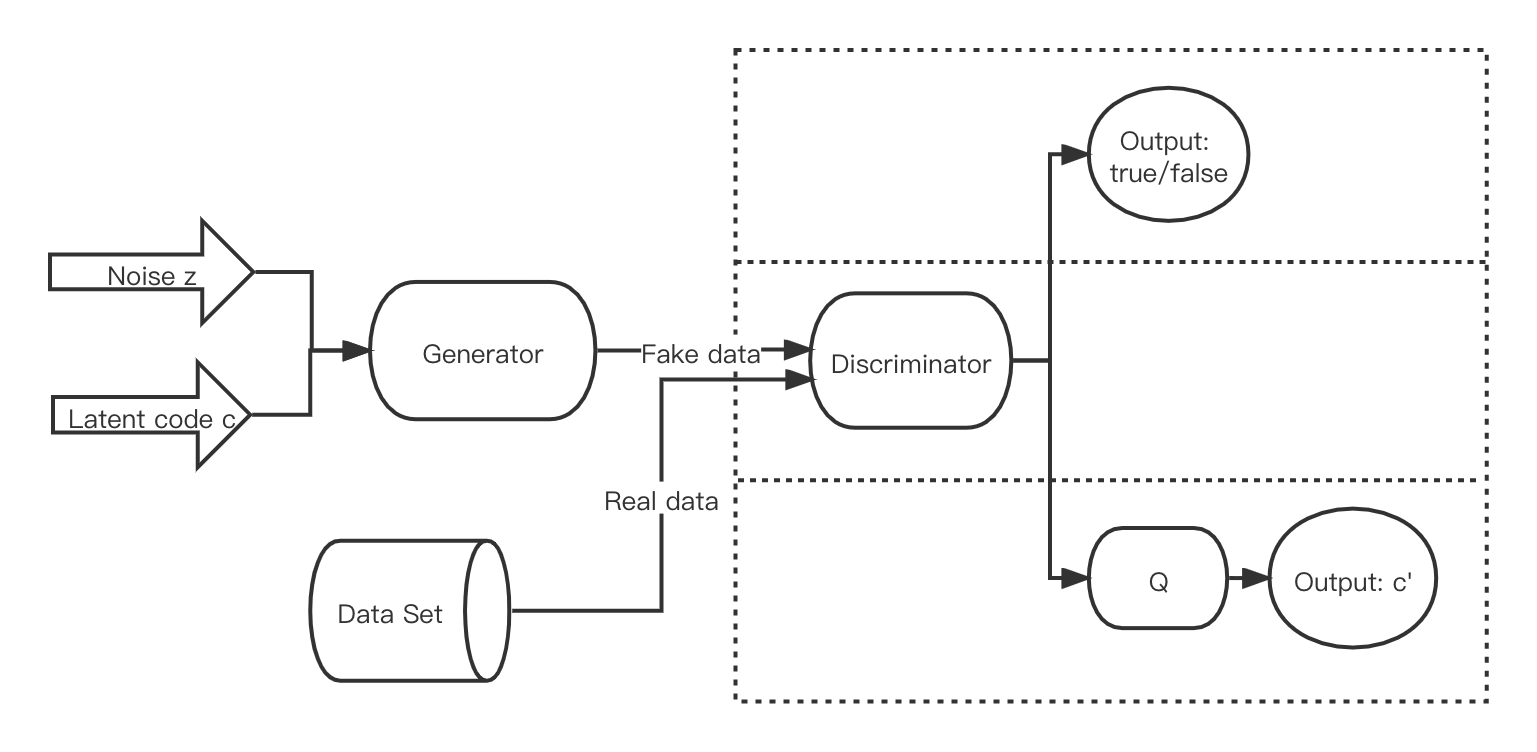
\includegraphics[width=\textwidth, height = 7cm]{figures/infoGAN.png}
  \caption{infoGAN Overview}{infoGAN consists of three parts, Generator G, Discriminator D and auxiliary network Q. D and Q share the network, only their last layers are different.}
%   \Description{infoGAN consists of 3 parts, Generator G, Discriminator D and auxiliary network Q. D and Q share the network, only their last layers are different.}
  \label{infoGan}
\end{figure*}

Based on the training result and latent code \(\mathbf{c}\), and the usage of the Generator to generate data and observe the characteristics of the generated data, we may deduce the information implied by \(\mathbf{c}\). The process of getting interpretable information from the input latent code is information disentanglement.

In our project, we will train the model using three integer latent codes and three continuous latent code. At every loop of the training of G, we modify the noise vector as the combination of an one-hot encoded vector with three random integer numbers and another vector with three random float numbers.

After the model is trained, we need to evaluate the latent codes by the method called latent traversal. Assume the discrete codes are \(\mathbf{C_1} = c_1, c_2, c_3\) and the continuous codes are  \(\mathbf{C_2}= c_4, c_5, c_6\). First we fix \(\mathbf{C_2}\) and set \(c_1 = 1, c_2 = 0, c_3=0\), then use the trained G to generate 10 trajectories. Then we draw 10 samples from the generated examples and plot the trajectories as pictures \(Pic_1\). Then fix \(\mathbf{C_2}\) and set \(c_1=0, c_2 = 1, c_3 = 0\) and generate 100 trajectories and take random 10 plot as pictures. We conduct the same process to each integer variables. Then we observe the trajectories in the picture and infer the possible factor that affects the trajectories. Our guess is speed and direction. We can start inferring  from these two factors. If we can find out the pattern in the trajectories, we can match them to the vector of integer latent codes. When evaluate the continuous codes, just fix the other two codes and change the one that is being evaluated by 0.1 every loop, the value of the code value should be in [0.1, 0.3, 0.5, 0.7, 0.9]. There will be \(3 \times 5 = 15\) groups of pictures. We observe the picture and try to deduce the factors from the trajectories.